\documentclass{article}

% if you need to pass options to natbib, use, e.g.:
% \PassOptionsToPackage{numbers, compress}{natbib}
% before loading nips_2016
%
% to avoid loading the natbib package, add option nonatbib:
% \usepackage[nonatbib]{nips_2016}

\usepackage[final]{nips_2016}
\usepackage{adjustbox}

% to compile a camera-ready version, add the [final] option, e.g.:
% \usepackage[final]{nips_2016}

\usepackage{amsmath,amsthm,amssymb}

\usepackage[utf8]{inputenc} % allow utf-8 input
\usepackage[T1]{fontenc}    % use 8-bit T1 fonts
\usepackage{hyperref}       % hyperlinks
\usepackage{url}            % simple URL typesetting
\usepackage{booktabs}       % professional-quality tables
\usepackage{amsfonts}       % blackboard math symbols
\usepackage{nicefrac}       % compact symbols for 1/2, etc.
\usepackage{microtype}      % microtypography

\title{Learning Senate Graph Structure}

% The \author macro works with any number of authors. There are two
% commands used to separate the names and addresses of multiple
% authors: \And and \AND.
%
% Using \And between authors leaves it to LaTeX to determine where to
% break the lines. Using \AND forces a line break at that point. So,
% if LaTeX puts 3 of 4 authors names on the first line, and the last
% on the second line, try using \AND instead of \And before the third
% author name.

\author{
  Horace Pan\\
  University of Chicago\\
  \texttt{hopan@uchicago.edu} \\
}

\begin{document}
% \nipsfinalcopy is no longer used

\maketitle

\begin{abstract}
We attempt to fit a graphical model to Senate roll call data from the 114th Congress(2015-2016) to
reveal information about Senators voting tendencies. We apply neighborhood selection and the graphical
lasso to learn the edge set of this graphical model.
\end{abstract}

\section{Introduction}

\section{Problem Setup}
Given $n$ samples of a $p$-dimensional multivariate Gaussian random variable $\mathbf{X} = (X_1, X_2, ..., X_p) \sim \mathcal{N}(\mu, \Sigma)$,
we want to learn the conditional independencies of the distribution. As we've seen in class, this can be
be represented with a graphical model, $\mathcal{G} = (V, E)$, where our vertex set is $V= \{1, 2, ..., p\}$ and our edge set
contains the edge $(i, j)$ if and only if $X_i$ is conditionally dependent on $X_j$ given the remaining variables. Every pair that is
not in our edge set are conditionally independent given the remaining variables. This is a well studied problem and many methods have been proposed over the years to solve it. In particular, we discuss two prevailing methods from the graphical model literature Neighborhood Selection and the Graphical Lasso in the following sections.

\section{Neighborhood Selection}
The idea of Neighborhood Selection is that the value of a single node 
should be dependent on only its neighbors. So, if we regress a single variable $X_i$ on the remainng
variables, we get the following coefficient vectors for $i=1, ..., p$: 
$$\Theta^{(i)} = \underset{\Theta: \Theta_i = 0}{argmin} || \mathbf{X}_{:,i} - X \Theta||_2^2 + \lambda ||\Theta||_1$$
Slightly deviating from the notation earlier, $\mathbf{X} \in \mathbb{R}^{n \times p}$, where $n$ is the number of samples and $p$ is the dimension of our random variable. $\mathbb{X}_{:, i}$ denotes the $i$th column of our data. The support of each coefficient vector can then be used to construct our edge set - the neighbors of vertice $i$ are exactly the $j$ indices where $\Theta_j^{(i)} \not = 0$. 
The Lasso penalty is used to encourage sparsity in our graphical model; having too many edges makes the graphical model less interpretable. 
Concretely, if we had a graphical model where all Republican senators clustered together, this would not tell us anything about their voting patterns(unless it were actually true that all Republican senators voted the same way every time).

\section{Graphical Lasso}
It is commonly known that the precision matrix(or the inverse covariance matrix) is informative of the
edge set of our graphical model. $\Sigma^{-1}_{i, j} = 0$ implies that variables $X_i$ and
$X_j$ are conditionally independent and that there is no edge between $X_i$ and $X_j$. So we can learn
the edge set of our graphical model by estimating the precision matrix. To do so, we solve for the precision
matrix that gives us the maximum log likelihood of our data.
$\Theta = argmax \log \det \Theta - tr(S \Theta) - \lambda ||\theta||_1$. In the following, $\mathbf{X}_i$ denotes the $ith$ sample.
\begin{proof}
Let $S$ be our empirical covariance: $S = \sum_{i=1}^n (\mathbf{X}_i - \mu)(\mathbf{X}_i - \mu)^T$
\begin{flalign}
P(\mathbf{X}|\mu) &= \frac{\det \Theta}{(2\pi)^{n/2}} \exp \frac{1}{2} (\mathbf{X} - \mu)^T \Theta (\mathbf{X}- \mu) \\
&= \frac{\det \Theta}{(2\pi)^{n/2}} \exp \frac{1}{2} (X - \mu)^T \Theta (X- \mu) \\
\log P(\mathbf{X}_1, \mathbf{X}_2, ..., \mathbf{X}_n | \mu) \propto \log \Pi_{i=1}^n P(\mathbf{X}_i | \mu)
&= \frac{\log \det(\Theta)}{10} \sum_{i=1}^n (\mathbf{X}_i - \mu)^T\Theta (\mathbf{X}_i - \mu) \\
&= \frac{\log \det(\Theta)}{10} \sum_{i=1}^n (\Theta \mathbf{X}_i - \mu)^T (\mathbf{X}_i - \mu)  \\
&= \frac{\log \det(\Theta)}{10} \sum_{i=1}^n (\Theta S)  \\
&= \frac{\log \det(\Theta)}{10} \sum_{i=1}^n (S \Theta)  \\
\end{flalign}
\end{proof}
We use the fact that $tr(AB) = tr(BA)$ repeatedly to get from line (4) to (5).

Banerjee, et. al. 2008 describes a block coordinate descent algorithm to solve this minimization problem. For my experiments, I used the GraphicalLasso method implemented in the scikit-learn Python library instead of writing it from scratch due to the fickle nature of the block coordinate convergence.

\section{Senate roll call data}
I scraped Senate roll call data from 2015-2016 from the 114th Congress off of \href{https://www.govtrack.us/}{https://www.govtrack.us/}. This included 339 votes
in 2015 and 88 votes(as of June 3rd) in 2016. Roll call date included the votes(Yes, No, Not present) for each senator, time of vote, the bill or amendment that
the vote pertained to, and the subject area of the vote(IE: Taxation, healthcare, etc).
Since we dealt with the "Not present" votes by setting those votes to "No/Nay" because a Not present vote is effectively a "No/Nay" vote for the purpose of passing a bill. I also tried using Senator's party's majority vote to fill in missing votes, but there was little discernable difference in the resulting graphical model in both cases.

\subsection{Refining bills by topic}
We implicitly assumed that all Senator voting tendencies are uniform across all bills. However, it is not to difficult to imagine cases where this is not true. Senators from farming states are
highly unlikely to vote against any bill that might reduce farm subsidies, regardless of what their party might vote. 
It is natural to expect that voting dependencies would vary by the subject of each bill. So, we attempt to cluster bills by their topics and then try to learn a separate graphical model for each subset of bills. We applied Latent Dirichlet Allocation on the bill summaries of each bill voted on. See table \ref{tbl: lda} for the resulting topics and some of the top words for each topic.

\begin{table*}[]
\centering
\vspace{-10pt}
\caption{\label{tbl: lda}Topics and top words computed with LDA}
\begin{tabular}{c c c c c}
\hline
Energy      & Budget    & Military/National Defense & Education & Health \\
\hline
energy      & deficit   & funds                     & school           & sec \\
water       & raising   & dod                       & district         & health \\
doe         & spending  & defense                   & requirements     & 2017 \\
efficiency  & fy2016    & security                  & esea             & medicaid \\
heaters     & reserve   & national                  & charter          & payments \\
demand      & increase  & program                   & student          & medical  \\
\hline
\end{tabular}
\end{table*}
I did not realize that I could actually scrape bills' subject areas until after doing this LDA(since the govtrack.us site didn't have the subject areas through its website, but did expose it through its bulk data api). Table \ref{tbl: topics} shows the breakdown of the topics
\begin{table*}[]
\centering
\vspace{-10pt}
\caption{\label{tbl: topics}Top Subject Areas Count(given by govtrack.us)}
\begin{tabular}{c c c c c}
\hline
Topic      & Bill Count    \\
\hline
Economics and Public Finance              & 123\\ 
Energy                                    &  66\\
Nomination                                &  42\\
Armed Forces and National Security        &  37\\
Health                                    &  29\\
Education                                 &  29\\
Crime and Law Enforcement                 &  25\\
Transportation and Public Works           &  16\\
Emergency Management                      &  11\\
Taxation                                  &  10\\
Government Operations and Politics        &   9\\
International Affairs                     &   7\\
Environmental Protection                  &   6\\
Labor and Employment                      &   4\\
Finance and Financial Sector              &   3\\
Immigration                               &   3\\
Foreign Trade and International Finance   &   3\\
Agriculture and Food                      &   2\\
Civil actions and liability               &   1\\
Law                                       &   1\\
\hline
Total                                     & 427\\
\hline
\end{tabular}
\end{table*}
So the top topics given by LDA given by LDA seem to match the true topics reasonably well. LDA missed the nominations topic(also was not in the top 10), but I think this is because the bill summaries for Nominations votes were almost always only a sentence long(EG: "On the Nomination PN327: Paula Xinis, of Maryland, to be United States District Judge for the District of Maryland") where as bill summaries for clotures/passages/resolutions/etc mostly spanned multiple paragraphs. I applied neighborhood selection on Economics, Energy, and Armed Forces/National Security. The following figures show the resulting graphical models. For all of the graphs, I generated a graph using the Networkx python library with the resulting edge sets given by Neighborhood selection or Graphical Lasso and then exported a gexf file. To visualize the graphs, I used Gephi, an open source graph visualization software. In the visualizations, the distances betweenconnected components are irrelevant; only the edge sets matter.

\begin{figure} 
\caption{\label{fig: nbd55}Neighborhood Selection with $\lambda = 0.55$}
  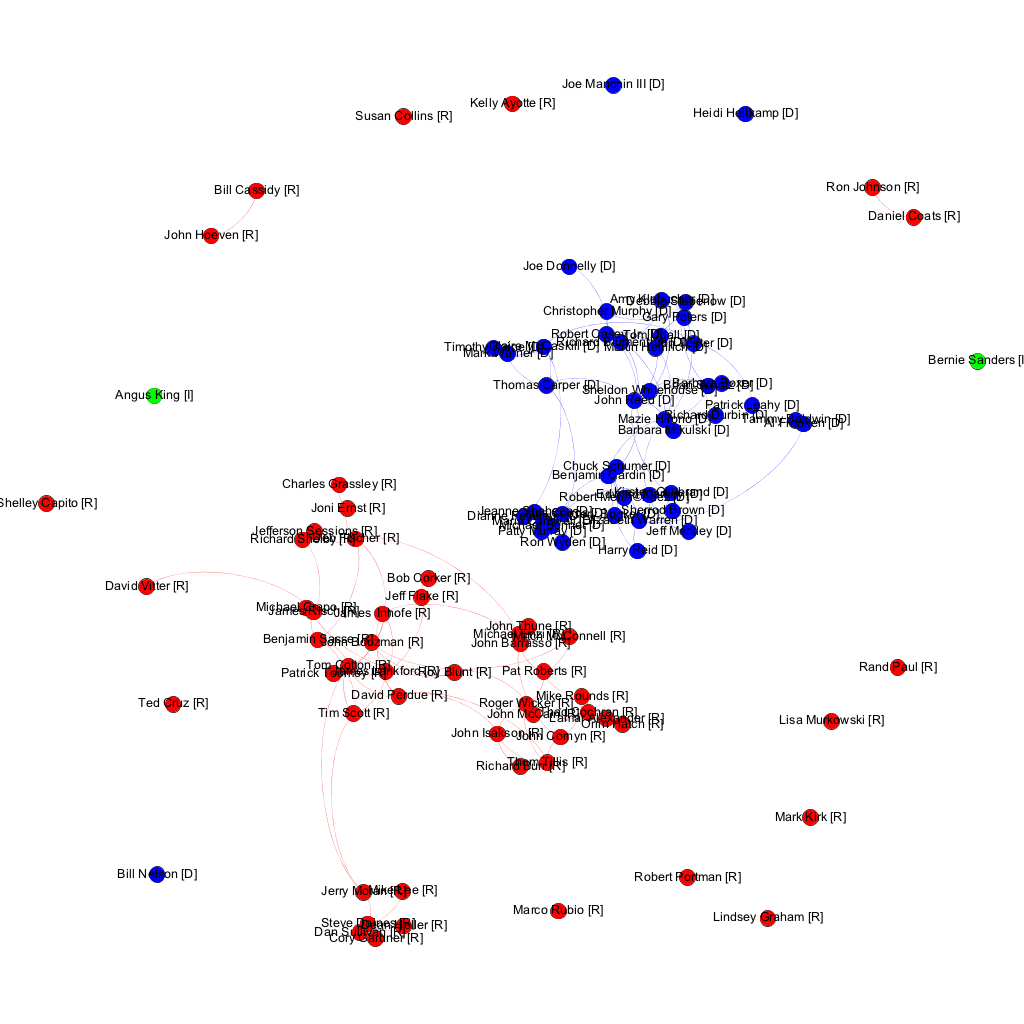
\includegraphics[width=\textwidth]{nbd_55_all.png}
\end{figure}

\begin{figure} 
\caption{\label{fig: nbd75}Neighborhood Selection with $\lambda = 0.75$}
  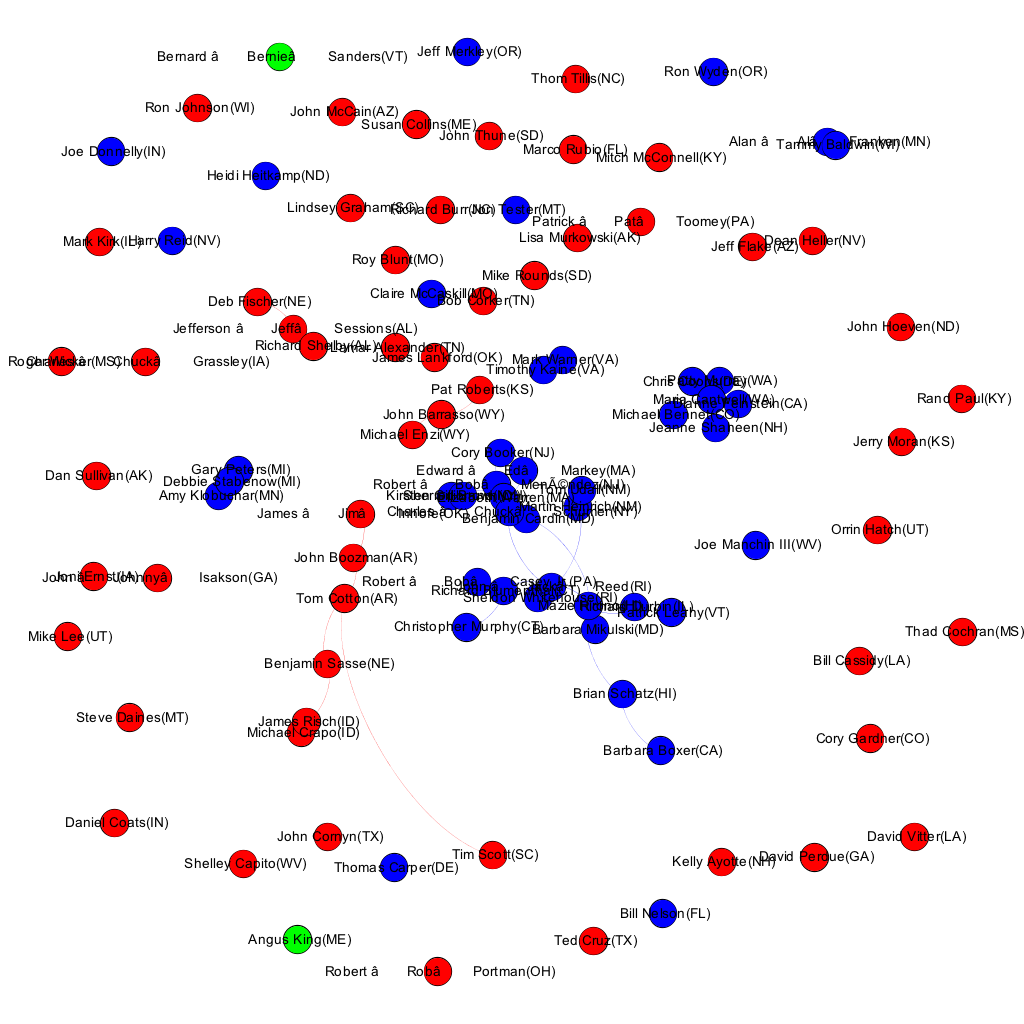
\includegraphics[width=\textwidth]{nbd_75.png}
\end{figure}

\section{Findings}
Figure 1 and 2 show the result of neighbhood selection applied with $lambda$ values of $0.55$ and $0..75$ respectively. In figure 1 we can see that the republican party(red) has
more "rogue" senators who have no dependencies on other Republican senators. The Democrat party is more tightly clustered and only has 3 senators(Joe Manchin(WV), Bill Nelson(FL) and Heidi Heitkamp(ND)).  West Virginia and North Dakota are relatively conservative states that Mitt Romney carried in the 2012 election, Manchin and Heitkamp are not connected to other Democrats. I'm not sure what's going on with Bill Nelson though. Though a bit hard to see, Harry Reid is only incident on two other vertices/senators, which I found a bit surprising. On a second comb through the data, I discovered that Reid had missed 54 out of the 427 votes so that might account for this supposed lack of influence. 

In figure 2, after increasing the LASSO penalty, we see that there are almost no dependencies between Republican senators, but the Democrats are still clsutered together. I suppose this shows that the Democratic party is more idealogically cohesive perhaps?

\section{Further Exploration}
A natural next step would be to investigate how similarities in demographic and location might affect voting patterns and dependencies on senators. It would also probably be
informative to run this sort of visualization on members of congress. Neighborhood selection and graphical lasso applied to senate roll call data is a visualization/exploratory
data analysis tool for political pundits more than anything else. The visualized clusters from the generated graphs would certainly be more interpretable to someone who is more well versed in US politics.
\section{Code and Data}
Code and data are hosted on my github repository at \href{https://www.github.com/horacepan/senatevoting}{https://www.github.com/horacepan/senatevoting}.
\section*{References}
References follow the acknowledgments. Use unnumbered first-level
heading for the references. Any choice of citation style is acceptable
as long as you are consistent. It is permissible to reduce the font
size to \verb+small+ (9 point) when listing the references. {\bf
  Remember that you can use a ninth page as long as it contains
  \emph{only} cited references.}
\medskip

\small

[1] Alexander, J.A.\ \& Mozer, M.C.\ (1995) Template-based algorithms
for connectionist rule extraction. In G.\ Tesauro, D.S.\ Touretzky and
T.K.\ Leen (eds.), {\it Advances in Neural Information Processing
  Systems 7}, pp.\ 609--616. Cambridge, MA: MIT Press.

[2] Bower, J.M.\ \& Beeman, D.\ (1995) {\it The Book of GENESIS:
  Exploring Realistic Neural Models with the GEneral NEural SImulation
  System.}  New York: TELOS/Springer--Verlag.

[3] Hasselmo, M.E., Schnell, E.\ \& Barkai, E.\ (1995) Dynamics of
learning and recall at excitatory recurrent synapses and cholinergic
modulation in rat hippocampal region CA3. {\it Journal of
  Neuroscience} {\bf 15}(7):5249-5262.

\end{document}
